\chapter{La machine à courant continu}
Ces machines ne sont plus utilisées comme génératrices de puissances 
mais leurs capacité de réglage de vitesse nous pousse à les étudier. 
\textbf{Dynamo} est le nom donné à une génératrice à courant continu.

\section{Génération d'une tension continue}
	\subsection{Effet d'un collecteur}
	Pour voir une f.e.m. continue, il faut 
	\begin{enumerate}
	\item Un collecteur
	\item Augmenter le nombre de conducteurs actifs
	\end{enumerate}
	Le \textbf{collecteur} est un commutateur ayant pour but de 
	redresser la f.e.m. alternative\footnote{"En électrotechnique, 
	un collecteur commutateur rotatif est un organe permettant de 
	créer 	une connexion électrique entre une partie fixe (stator) 
	et une 	partie tournante (rotor), avec une fonction de 
	commutation pendant la rotation. On trouve ce genre de 
	collecteur dans les machines à courant continu et les moteurs 
	électriques universels.".}.\\
	\begin{wrapfigure}[10]{l}{8.2cm}
	\vspace{-5mm}
	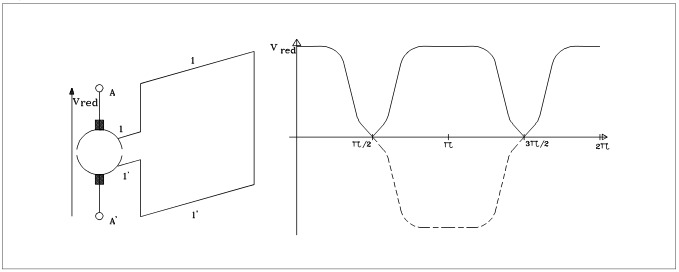
\includegraphics[scale=0.34]{ch4/image1.png}
	\captionof{figure}{ }
	\end{wrapfigure}
	\textbf{Petit plus (Source : Wikipedia) :} \textit{Ce collecteur 
	commutateur rotatif consiste en un anneau conducteur de l'électricité  
	sectionné en un nombre pair de parties 
	isolées entre elles, fixé avec une entretoise isolante sur l'axe de 
	la machine. La connexion électrique est créée entre les parties 
	conductrices et la partie fixée sur le stator (bornier), par une ou 
	plusieurs paires de balais positionnées respectivement à 180$\ ^\circ$. 
	On alimente en électricité le bobinage du rotor par ces contacts 
	(fonctionnement en moteur) ou au contraire on récupère l'électricité 
	produite par le bobinage du rotor (fonctionnement en générateur).}\ \\
	
	L'idée de l'espacement de $\pi$ est que le sens du courant dans 
	l'anneau conducteur va s'inverser, permettant au rotor de continuer 
	à tourner comme on peut le voir sur l'illustration ci-contre.\\
	On obtiendra aux balais une f.e.m. unidirectionnelle et dans le circuit 
	extérieur un courant unidirectionnel. Cependant, la grandeur ce cette 
	f.e.m. et du courant qui en résulte ne sont pas constantes.
	
	\newpage
	\begin{wrapfigure}[11]{r}{6.8cm}
	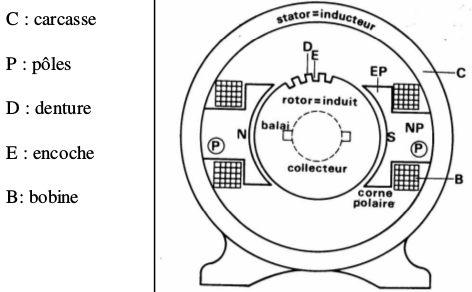
\includegraphics[scale=0.4]{ch4/image2.png}
	\captionof{figure}{ }
	\end{wrapfigure}
	Considérons un exemple "réel". Cette machine est constituée de 
	\begin{itemize}
	\item[$\bullet$] Un inducteur, sur le stator possédant $p$ paires de 
	pôles saillants. La répartition de l'induction dans l'entrefer a une 
	forme trapézoïdale avec comme axe de symétrie l'axe \textit{longitudinal} 
	$d$. L'axe électriquement $\perp$ à celui-ci est l'axe \textit{transversal},
	$q$.
	\item[$\bullet$] 	Un induit, disposés sous la forme d'enroulements de 
	conducteurs placés dans les encoches du cylindre rotorique. On connecte 
	via les faces latérales du cylindre ces conducteurs pour former un 
	\textit{enroulement en tambour.} 
	\end{itemize}\ 
	
	Les conducteurs actifs réunis par ces liaisons sont situés sous les 
	pôles opposés, d’où il résulte une addition des f.e.m. induites.
	La \textbf{commutation} d’une lame à l’autre se fait donc au moment 
	où un conducteur actif passe d’un pôle à l’autre
	
	
	\subsection{Machine multipolaire}
	On considérait jusqu'ici des machines à deux pôles inducteurs, soyons 
	fous et plaçons-en maintenant quatre. Par symétries, les f.e.m. seront 
	égales en grandeurs. Si l'on connecte les balais opposés entre eux (
	les deux négatifs ensemble, de même pour les positifs) on obtient une 
	dynamo multipolaire à \textit{enroulement parallèles}.
	
	\subsection{Types d'enroulement d'induit}
	Problème complexe non abordé ici. Sachez juste que pour l'enroulement 
	en tambour, on peut avoir l'enroulement \textit{imbriqué} ou l'
	enroulement \textit{ondulé}.
	
	\subsection{Tension à vide en régime statique}
	Soit un enroulement en tambour (l'armature, $a$) de $N_C$ conducteurs 
	répartis uniformément en deux couches. Le nombre de spires $N_S=N_C/2$. 
	On va supposer l'induit infiniment divisé de sorte à avoir une densité 
	linéique de spires $N_S/(2\pi R)$. On suppose un rotor lisse.
	
		\subsubsection{Méthode des champs}
		\begin{wrapfigure}[11]{l}{4.8cm}
		\vspace{-5mm}
		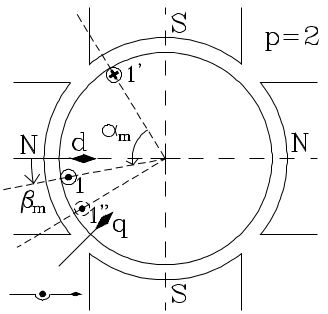
\includegraphics[scale=0.4]{ch4/image3.png}
		\captionof{figure}{ }
		\end{wrapfigure}
		Soit une spire constituée d'un conducteur d'entrée 1 et de sortie 
		1'. Nous avons
		\begin{description}
		\item[$\beta_m$ :] la coordonnée angulaire mécanique de l'entrée 1
		\item[$\beta_m-\alpha_m$ :] la coordonnée mécanique de sortie 1'
		\end{description}				
		La f.e.m. engendrée dans la spire vaut (voir figure ci-contre pour 
		la convention de signe (conducteur entrant et sortant))
		\begin{equation}
		\begin{array}{ll}
		e_{spire} &= B(\beta_m)lv - B(\beta_m-\alpha_m)lv\\
		&= (B(\beta_m)-B(\beta_m-\alpha_m))lv
		\end{array}
		\end{equation}
		Si $\alpha_m = \pi/p$ la spire est \textit{diamétrale}. Le "sens" 
		du champ $B$ sera donc exactement opposé
		\begin{equation}
		\begin{array}{l}
		B(\beta_m-\alpha_m) = - B(\beta_m)\\
		\hookrightarrow e_{spire} = 2B(\beta_m)lv
		\end{array}
		\end{equation}
		Si $\alpha_m<\pi/p$ on parle de spire \textit{à pas raccourci} : 
		on définit 1" déphasé de $\pi/p$ en avant par rapport à 1' et 
		donc déphasé de $\delta_m = \pi/p-\alpha_m$ par rapport à 1. Par 
		symétrie\footnote{??}
		\begin{equation}
		 \begin{array}{ll}
		B(1') = -B(1")\qquad\text{ou}\qquad B(\beta_m-\alpha_m) &=-B(\beta_m
		-\alpha_m+\frac{\pi}{p})\\
		&=-B(\beta_m+\delta_m)		
		\end{array}
		\end{equation}
		Impliquant que $e_{spire} = e_1-e_{1'}=e_1+e_{1"}$, en considérant 
		$B>0$ sous la pôle nord.\\
		On peut alors avoir une répartition rectangulaire de l'induction
		\begin{center}
		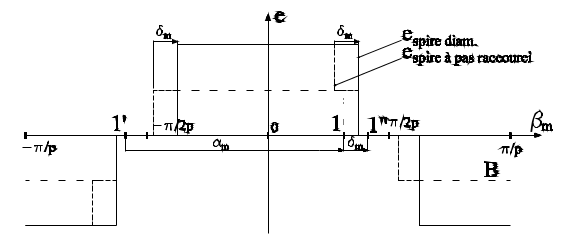
\includegraphics[scale=0.5]{ch4/image4}
		\end{center}
		ou  trapézoïdale 
		\begin{center}
		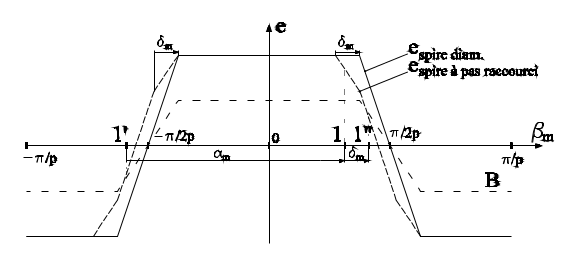
\includegraphics[scale=0.5]{ch4/image5}
		\end{center}
		
		\textsc{Forces électromotrice entre balais}\ \\
		\begin{wrapfigure}[12]{l}{6cm}
		\vspace{-2mm}
		\begin{equation}
		\begin{array}{ll}
		e &= \displaystyle p \int_{-\frac{\pi}{2p}}^{\frac{\pi}{2p}} 
		e_{spire}.\text{densité de spire}\\
		&= \displaystyle p \int_{-\frac{\pi}{2p}}^{\frac{\pi}{2p}} (
		2B(\beta_m)kv)\frac{N_s}{2d\pi}\ d\beta_m\\
		&= \displaystyle \frac{p}{d}N_s\frac{\Omega_r}{\pi} \int_{-
		\frac{\pi}{2p}}^{\frac{\pi}{2p}}B(\beta_m)lR\ d\beta_m\\
		&= \displaystyle\frac{p}{d}N_s\frac{\Omega_r}{\pi}\Phi
		\end{array}
		\end{equation}

		\end{wrapfigure}
		Supposons un enroulement à spires diamétrales tel que $e_{spire} = 
		2B(\beta_m)lv$. La f.e.m. entre balais est constante si l'induit 
		est infiniment divisé. Considérons un enroulement ondulé à $2d$ 
		dérivations : une dérivation comporte $N_S/(2d)$ spires. Celle-ci 
		est constitués par des spires dont les conducteurs d'entrée et 
		de sorties sont sous des pôles de même signe, il y a donc 
		$(N_S/2d).(1/\pi)$ spires appartenant à une dérivation par rad. 
		mécanique. Pour obtenir la tension aux bornes de la dérivation, 
		il faut intégrer les tensions de chaque spire de la dérivation. 
		Comme il y a $p$ paires de pôles, il convient de multiplier le 
		résultat d'un pôle par $p$. De façon générale :\\
		
		\retenir{\begin{equation}
		e = K\ \Omega_r\ \Phi
		\end{equation}
		où	$\Phi$ est le flux utile (coupé par une spire diamétrale 
		d'axe longitudinal de l'induit) par pôle, $\Omega_r$ en rad/s et 
		$K$, une constante qui dépend des données de l'enroulement.}
		
		\newpage
		\begin{wrapfigure}[12]{l}{4.8cm}
		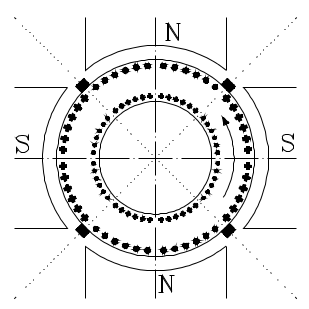
\includegraphics[scale=0.4]{ch4/image6.png}
		\captionof{figure}{ }
		\end{wrapfigure}
		La f.e.m. (tension à vide) d'une dynamo est $\propto$ au flux 
		utile par les pôles et la vitesse de rotation. Cette formule 
		reste valable pour une machine en charge ($i_a\neq0$) si on 
		considère que $\Phi$ pourrait être modifié par $i_a$. $\Phi$ 
		dépend de $i_e$ de façon non-linéaire (cf. labo).\\
		
		Ci-contre, la répartition des f.e.m. engendré pour une dynamo 
		à induit infiniment divisé de spires diamétrales. La tension 
		entre deux balais est la somme ($\int$) de toutes les f.e.m. 
		sous un même pôle. Ce schéma confirme que la f.e.m. est bien 
		alternative mais constante en un point fixe : 
		\textbf{pseudo-stationnaire} du à l'effet redresseur du 
		collecteur.

		\subsubsection{Méthode des circuits}
		\begin{wrapfigure}[1]{r}{2.8cm}
		\vspace{-5mm}
		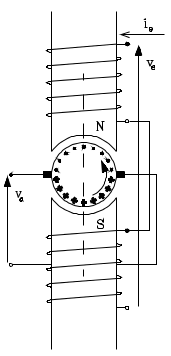
\includegraphics[scale=0.5]{ch4/image7.png}
		\captionof{figure}{ }
		\end{wrapfigure}
		Soit deux enroulements : un d'excitation parcouru par $i_e$ 
		et un induit pseudo-stationnaire à vide. A bornes du balais, 
		on a donc
		\begin{equation}
		v_a = R_ai_a+D\Psi_a
		\end{equation}
		où $\Psi_a$ est le flux coupé par l'enroulement induit, flux 
		créé par le courant d'excitation. On peut écrire
		\begin{equation}
		\Psi_a = M(\beta_m,i_e)i_e
		\end{equation}
		où $M$ est l'inductance mutuelle entre les enroulement $e$ 
		et $a$, mutuelle fonction de $\beta$, l'angle de décalage 
		entre $N$ et l'axe d'enroulement. En faisant les math ;
		\begin{equation}
		\begin{array}{ll}
		(v_a)_{i_a=0} &= \displaystyle D\Psi_a\\
		&= \displaystyle D(Mi_e)\\
		&= \displaystyle  DM\ i_e + M\ Di_e\\
		&= \displaystyle \frac{\partial M}{\partial \beta_m}D\beta_m
		i_e + \frac{\partial M}{\partial i_e}Di_e i_e + M\ Di_e\\
		&= \displaystyle G(\beta_m,i_e)\Sigma_r i_e +\left(M+\frac{
		\partial M}{\partial i_e}i_e\right)Di_e
		\end{array}
		\end{equation}
		On définit alors la valeur locale (ou différentielle) de la 
		mutuelle : $\displaystyle M' = M+\frac{\partial M}{\partial 
		i_e}i_e$, qui sera nulle si les balais sont calés sur l'axe 
		neutre ($\beta = \pi/2$) car $a \perp e$. \\
		On définit également la \textbf{fonction d'excitation}
		\begin{equation}
		G(i_e) = \frac{\partial M(\beta_m,i_e)}{\partial \beta_m}) =
		\frac{(\partial \Psi_a/\partial \beta_m)}{i_e}\qquad si\qquad 
		\beta=\frac{\pi}{2}, i_e=\text{ cste}
		\end{equation}
		La f.e.m. vaut alors $e = (v_a)_{i_a=0} = G(i_e)i_e\Omega_r$ 
		qui ressemble à notre belle formule encadré plus haut ! On 
		peut dès lors écrire
		\begin{equation}
		G(i_e)i_e = K\Phi
		\end{equation}
		La connaissance de la caractéristique à vide qui conduisait 
		immédiatement à la détermination de $K, \Phi$ en fonction de 
		$i_e$, il en est de même pour $G$ en fonction de $i_e$.
		
	\newpage
	\subsection{Effet de décalage des balais}
	\begin{wrapfigure}[7]{r}{9.5cm}
	\vspace{-8mm}
	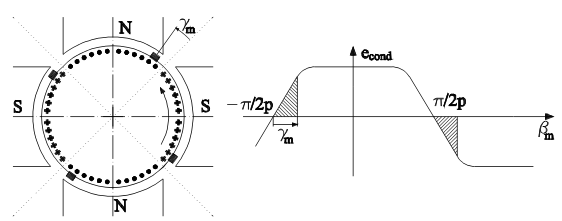
\includegraphics[scale=0.5]{ch4/image8.png}
	\captionof{figure}{ }
	\end{wrapfigure}
	Dans l'expression de la tension à vide, on a maintenant comme 
	limites $-\frac{\pi}{2}p+\gamma_m$ et $\frac{\pi}{2}p+\gamma_m$ (à 
	la place de $-\frac{\pi}{2}p+$ et $\frac{\pi}{2}p$), réduisant la 
	valeur de celle-ci par rapport à leurs positions sur les axes neutres. 
	Il faut encore rajouter à ça un effet de mutuelle.
	
	\subsection{Tension à vide - modèle mathématique}
	Trois remarques sur ce qu'est un bon modèle
	\begin{enumerate}
	\item Adapté au but poursuivi, ça ne sert à rien de faire trop.
	\item Il doit être simple, sinon avoues que tu ne le liras pas.
	\item Il doit être homogène, si on applique un hypothèse il faut 
	toujours l'appliquer.
	\end{enumerate}\ \\
	
	\textsc{Exemple - dynamo à vide}\\
	Définissions comme variables de commande $v_e$ la tension aux bornes 
	du circuit d'excitation, $\Omega_r$ la vitesse de rotation et $e$, 
	la tension à vides aux bornes des balais comme variable de sortie. 
	Connaissant deux expressions pour $e$, il suffit d'en prendre une et 
	de la compléter par l'équation du circuit d'excitation pour obtenir le 
	modèle recherché : $v_e = R_ei_e +D\Psi_e$.
	
		\subsubsection{Modèle non-linéaire}
		Il suffit d'utiliser une relation non-linéaire entre $\Psi_e$ 
		et $i_e$ pour compliquer le tout : $\Psi_e = L_e(i_e)i_e$ où 
		$L_e$ est l'inductance propre du circuit d'excitation, fonction 
		non-linéaire. Si l'on considère que $\Psi_e$ est variable d'état :
		ré-écrivons notre équation sous la forme d'une ED :
		\begin{equation}
		D\Psi_e = v_e-R_ei_e(\Psi_e)
		\end{equation}
		Si cette fois on choisi $i_e$ comme variable d'état, on peut 
		écrire
		\begin{equation}
		\dfrac{\partial \Psi_e}{\partial i_e}Di_e = v_e-R_ei_e\quad 
		\Longrightarrow\quad Di_e = \dfrac{v_e - R_ei_e}{L_e'}
		\end{equation}
		où $L_e'(i_e)$ est la valeur différentielle de l'inductance 
		propre du circuit $e$. Notons qu'elle est aussi égale à 
		$L_e+(\partial L_e/\partial i_e)i_e = \partial\psi_e/\partial 
		i_e$. Sachant que $e = (v_a)_{i_a=0} = G(i_e)i_e\Omega_r$, le 
		calcul de $e$ est immédiat si l'on a $i_e$.\\

		\begin{wrapfigure}[6]{l}{7cm}
		\vspace{-8mm}
		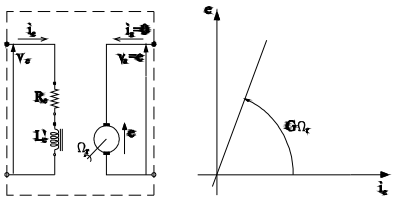
\includegraphics[scale=0.5]{ch4/image9.png}
		\captionof{figure}{ }
		\end{wrapfigure}
		Nos deux équations trop stylées 
		\begin{equation}
		\begin{array}{ll}
		v_e &= R_ei_e + L_e Di_e\\
		e &= K\Phi\Omega_r = G\Omega_ri_e
		\end{array}
		\end{equation}
		nous fournissent un schéma équivalent dont la caractéristique 
		permet le passage de $\Psi_e$ à $i_e$.
		
		\newpage
		Il est également possible, via $D\Psi_e = v_e - R_ei_e(\Psi_e)$ 
		d'obtenir le schéma-bloc suivant :
		\begin{center}
		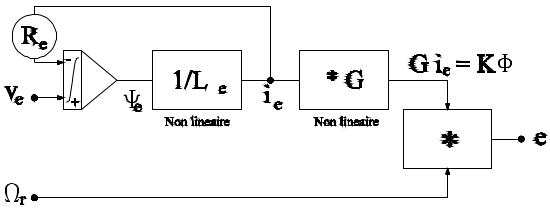
\includegraphics[scale=0.5]{ch4/image10.png}
		\captionof{figure}{ }		
		\end{center}			
		
		\subsubsection{Modèle linéaire}
		On peut l'obtenir en considérant de "petits mouvements" et en 
		substituant les courbes par leurs tangentes. Supposons que 
		$L_e = L_e' = L_{e,ns} = \text{cste}$ et $G = G_{ns} = 
		\text{cste}$. Notre précédente relation devient alors 
		\begin{equation}
		Di_e = \frac{v_e - R_ei_e}{L_e} \quad \lt\quad I_e(p) : 
		\frac{1}{1+pT_e}\frac{V_e(p)}{R_e}
		\end{equation}
		où $T_e = L_e/R_e$ est la constante de temps du circuit d'
		excitation (valeur assez élevée comme beaucoup d'enroulements). 
		Cette relation obtenue via Laplace est assez évidente à vue 
		du schéma équivalent, car ce-dernier est constitué de $R_e$ 
		et $L_e$. La grandeur de sortie vaut toujours 
		\begin{equation}
		e = Gi_e\Omega_r
		\end{equation}
		et dépend linéairement de $i_e$ si la vitesse est constante. 
		Le système global est du premier ordre
		\begin{equation}
		E(p) = G\Omega_r I_e(p) = G\Omega_r \dfrac{1}{1+pT_e}\frac{V_e
		}{R_e}
		\end{equation}
		\begin{center}
		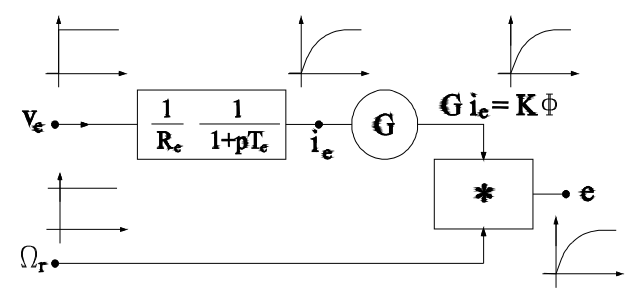
\includegraphics[scale=0.5]{ch4/image11.png}
		\captionof{figure}{ }		
		\end{center}			
		
			
\section{Influence du courant d'armature}
En effet, ça on sent que la machine en charge comportera en plus d'une 
source de tension une résistance $R_a$ et une inductance $L_a$.

	\subsection{Effet Joule (résistance $R_a$)}
	On les trouve dans l'enroulement ainsi que dans le ballais/collecteur,
	dépendant de plusieurs paramètres tel que la température et la valeur du courant.
	Mesurer la résistance globale n'est pas aisé, la résistance n'étant 
	pas la même quand la machine est en fonction ou non : en rotation, 
	elle est perturbée par la f.e.m. rémanente. En gros, les chutes sont 
	\begin{equation}
	\Delta V_{R_a} = \Delta V_b\text{sign}(i_a) + R_ai_a
	\end{equation}
	où $\Delta V_b$ représente la chute balais collecteur (fonction du 
	sens de rotation) et $R_a$ la résistance entre enroulements. Par 
	\textbf{convention}, la chute est fixée à $2V$ pour les balais en 
	carbone et $0.6V$ pour les métalliques.
	
	\subsection{Réaction transversale de l'armature infiniment divisée}
	\begin{wrapfigure}[9]{l}{4.7cm}
	\vspace{-5mm}
	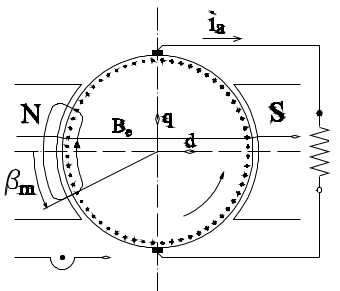
\includegraphics[scale=0.34]{ch4/image12.png}
	\captionof{figure}{ }
	\end{wrapfigure}
	Soit une génératrice avec un courant infiniment divisé qui circule 
	dans l'induit, même sens que la f.e.m. Les courants induits créent 
	à leurs tour un champ créant un flux perpendiculaire au flux 
	inducteur. En désignant $\beta_m$ l'abscisse angulaire d'un point, 
	calculons les ampères-tours dans un contour d'induction fermé :
	\begin{equation}
	\frac{N_c}{2\pi}\frac{i_a}{2d}2\beta_m
	\end{equation}
	Par symétrie par rapport à l'axe des pôles, la moitié des A.t. est 
	attribué à la moitié du chemin. Par abus, on attribue des A.t. la 
	ou le chemin traverse l'entrefer. Si ce dernier est constant et le 
	fer parfait 
	\begin{equation}
	H(\beta_m) = \frac{N_c}{2\pi}\frac{i_a}{2d}\frac{\beta_m}{\delta}
	\end{equation}
	$H$ est max si $\beta_m=\pi/2p$ : 
	\begin{equation}
	H\left(\frac{\pi}{2p}\right) = \frac{N_c}{2\pi}\frac{i_a}{2d}\frac{
	\pi}{2p\delta} = \frac{N_c}{8\delta}\frac{i_a}{pd}=\frac{N_s}{4\delta}
	\frac{i_a}{pd}
	\end{equation}
	Si le fer est réel il suffit de multiplier par $\mu_0$. Tout ceci 
	est bien indépendant de la vitesse de rotation : la situation est 
	la même que si une bobine était alignée sur l'axe neutre.
	
		\begin{center}
		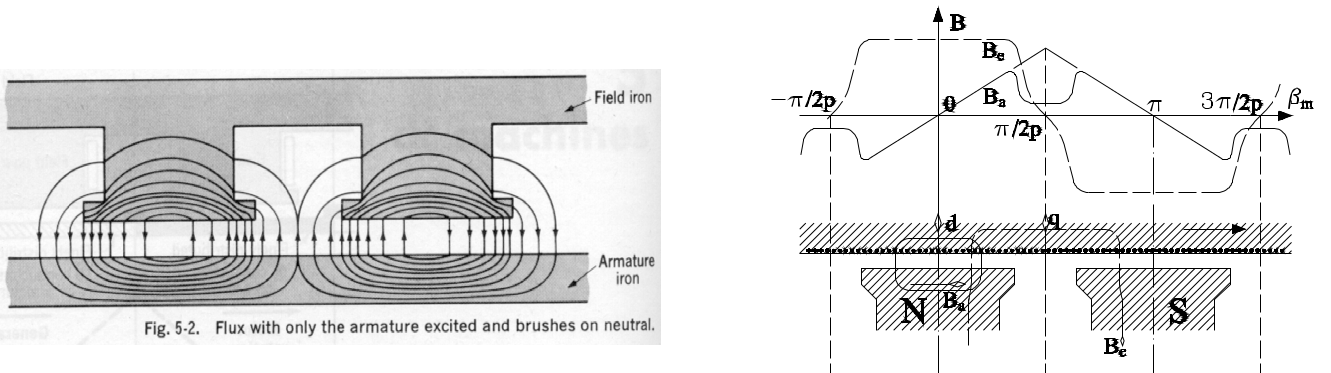
\includegraphics[scale=0.35]{ch4/image13.png}
		\captionof{figure}{ }		
		\end{center}
	
	Pour calculer $L_a$ on considère un enroulement fictif dont toutes 
	les spires ont par axe celui du balai : le flux vaudra l'intégrale 
	de l'induction entre $\beta_m et \pi-\beta_m$. Grâce au flux 
	totalisé : $L_a=\Psi_a/i_a$.
	
	\subsection{Le champ résultant}
		\subsubsection{Sans saturation}
		\begin{wrapfigure}[7]{r}{4.7cm}
	\vspace{-25mm}
	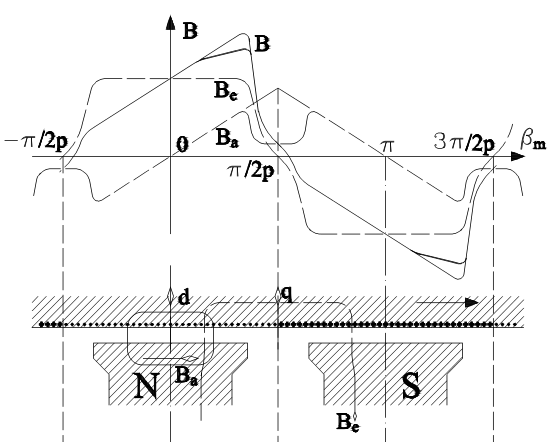
\includegraphics[scale=0.34]{ch4/image14.png}
	\captionof{figure}{ }
	\end{wrapfigure}
		On peut appliquer le principe de superposition. Pour une dynamo, 
		une fois la réaction d'induit est magnétisante (corne d'entrée) 
		et une fois démagnétisant (corde de sortie). La figure ci-contre 
		montre comment obtenir $B$ par la somme de l'induction de l'inducteur 
		$B_e$ et la réaction d'induit $B_a$.\\
		Notons que le flux n'a pas changé, la f.e.m. en charge est la 
		même qu'à vide.
		
		\subsubsection{Avec saturation}
		L'induction en charge est plus petite que la somme de l'excitation 
		et la réaction d'induit. Le flux longitudinal est plus faible, 
		causant une f.e.m. plus faible $\rightarrow$\textit{ La réaction 
		d'induit possède une composante longitudinale à cause de la 
		saturation.}. Pour décrire l'effet démagnétisant, trois hypothèses :
		\begin{enumerate}
		\item Lignes de forces radiales dans l'entrefer.
		\item L'induction null en dehors des pôles.
		\item Démonstration faite pour $p=d=1$.
		\end{enumerate}
		A vide, juste avec le courant d'excitation $i_e$ on a $A.t._e = 
		N_ei_e$. Si la spire n'est pas sous le pôle sa tension est nulle. 
		Si par contre elle est sous le pôle elle sera $\propto B_e$. La 
		courbe a vide donne le lien entre $e$ et $N_ei_e$ mais aussi la 
		f.e.m. à une constante près.\\
		Les courants induits causent également des A.t. de réactions 
		d'induits qui varient linéairement entre la corne de sortie $-A$ 
		et d'entrée $+A$ de la sorte :
		\begin{equation}
		A = \frac{N_c}{2\pi}\frac{i_a}{2}\frac{b_i}{4\pi R}
		\end{equation}
		Les A.t. varient ainsi linéairement de $N_ei_e-A$ à $N_ei_e+A$ (
		$OP_1$ à $OP_2$ sur le schéma page 4.33). \textbf{Lire le texte 
		sur cette page, c'est assez confus.}
		
		\subsubsection{Couple électromécanique - Couple extérieur}
		La loi de Laplace ($F+ilB$) permet de calculer la somme sur 
		chaque conducteur pour ensuite les sommer, mais il est plus 
		simple d'utiliser la conservation de la puissance : la somme 
		de la puissance appliquée électriquement et de la puissance 
		appliquée mécaniquement est nulle\footnote{? (en convention 
		récepteur)} :
		\begin{equation}
		[\underbrace{P_{electrique} - (P_{pJoule}}_{P_{electromecanique}}
		+P_{pmagn})] + [P_{mecan}-P_{meca}]=0
		\end{equation}
		où les pertes joules $P_{pJ}=0$ si $î_a=0$. Par contre les pertes 
		magnétiques existent tout de même (hystérèse, Foucault, ...). Les 
		pertes méca sont dues aux frottement (fonction de $\Omega_r$). La 
		puissance mécanique appliquée à un moteur est négative. On peut 
		calculer le couple électromécanique $P_{em} = C_{em}\Omega_r$.
		
		
		
		
		
		
		
		
		
		
		
		
